\documentclass[letterpaper]{article}

\usepackage[english]{babel}
\usepackage[utf8]{inputenc}
\usepackage{amsmath}
\usepackage{graphicx}
\usepackage[colorinlistoftodos]{todonotes}
\usepackage[]{algorithm2e}
\usepackage{listings}
\usepackage{hyperref}
\usepackage{float}
\usepackage{afterpage}

\newcommand\blankpage{%
	\null
	\thispagestyle{empty}%
	\addtocounter{page}{-1}%
	\newpage}

\title{CSCE 689: Cloud Computing}
\author{Aryan Sharma (UIN: 326006767)}

\date{\today}

\begin{document}
%\maketitle
%\newpage

\begin{titlepage}
	\centering
	%\includegraphics[width=0.15\textwidth]{example-image-1x1}\par\vspace{1cm}
	{\scshape\LARGE Texas A\&M University \par}
	\vspace{1cm}
	{\scshape\Large CSCE 689: Cloud Computing\par}
	\vspace{1.5cm}
	{\huge\bfseries Homework I\par}
	\vspace{2cm}
	{\Large Aryan Sharma \par}
	{\normalsize UIN: 326006767 | aryans@tamu.edu\par}
	\vfill
	
	% Bottom of the page
	{\large \today\par}
\end{titlepage}

\tableofcontents
%\afterpage{\blankpage}

\newpage

\section{Task I}
\label{sec:introduction}

This task is to assist the AggieFit team in designing their system by providing prototypes and comments.

\subsection{Time Taken}

The time taken to achieve this task was 6 hours. I used the \textit{virtualenv} command to setup a new virtual environment so that the dependencies are inplace. I used Python 2.7 version and the latest versions of MongoDB. 

\subsection{Task 1a}

The relational database has been the foundation of enterprise applications for decades, and has been a popular and inexpensive option. Today, database designers are thinking about better ways to store and manage their data and many of the assumptions that drove the development of earlier relational databases have changed, like here in in the scenario of Aggiefit.

MongoDB is an open-source, non-relational database which stores data as documents in a binary representation called BSON (Binary JSON). Related information is stored together for fast query access through the MongoDB query language. Fields can vary from document to document; there is no need to declare the structure of documents to the system - documents are self-describing. If a new field needs to be added to a document, then the field can be created without affecting all other documents in the collection, without updating a central system catalog, and without taking the system offline. Optionally, schema validation can be used to enforce data governance controls over each collection.

Hence, MongoDB would enable us to build the applications, handle highly diverse data types, and manage the application more efficiently at scale. Development is simplified as MongoDB documents map naturally to modern, object-oriented programming languages. Using MongoDB removes the complex object-relational mapping (ORM) layer that translates objects in code to relational tables. MongoDB’s flexible data model also means that your database schema can evolve with business requirements. MongoDB, in contrast to RDMBMS (like MySQL) can also be scaled within and across multiple distributed data centers as our deployments grow in terms of data volume and throughput.

Hence, for Aggiefit MongoDB turns out to be a good choice as we have the options to scale our database for future users, Besides, it being schemaless, we have the option to store the table entites as we want without affecting other entities (or documents in MongoDB). This also works well for distributed computing as MongoDB is distributed database.  

\subsection{Task 1b}

Some of the queries which require calculations from our databases can be precomputed and cached. This would save our time when we trying to compute it on the fly. Besides, we can add another data entry \textit{Status} to store whether the user of the application is active or not. In case he is active we can set this data entry to 0, without loosing (by deletion) his existing data. In case he wants to continue the applicaition we can simply set that status field to 1 and the need to enter his data again would not be necessary.

\subsection{How to run the code}

The queries are written in the file \textit{queries.py}. It can be run on the terminal as \textit{python queries.py}. 

For the part WQ1 and WQ2, the entire databases are dumbed for comparison. For the rest parts, the UID is printed along with the value, if any. The snapshot is shown in Fig. 1.  

\begin{figure}
	\centering
	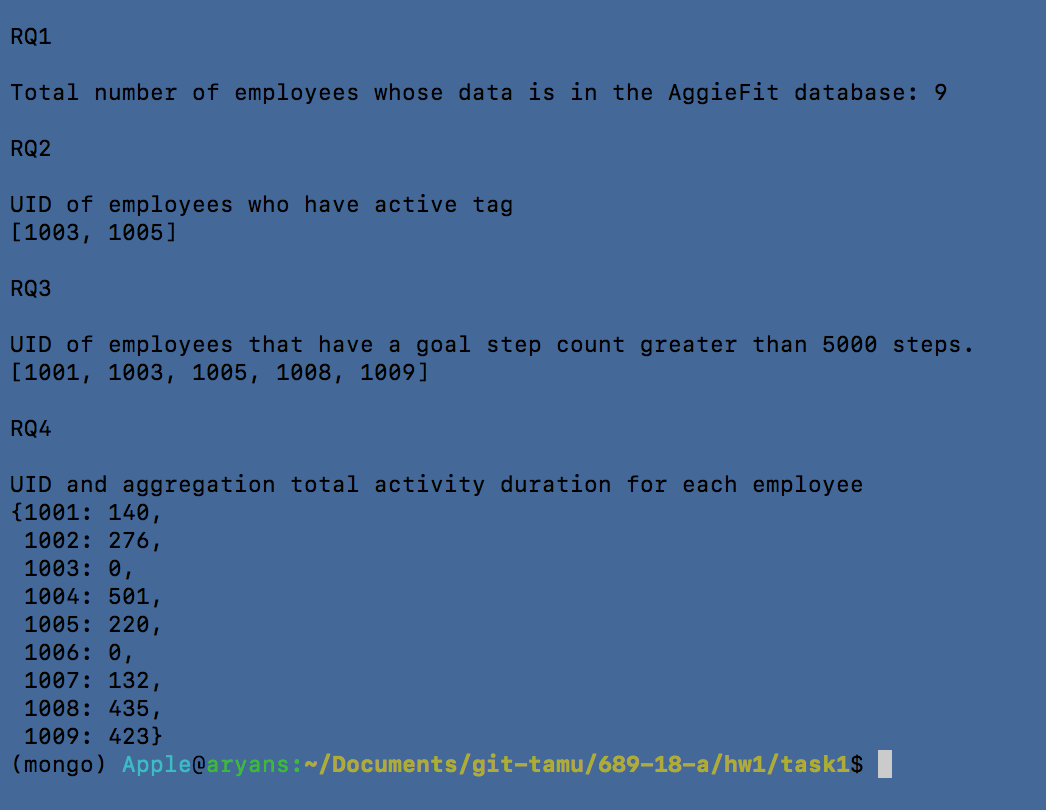
\includegraphics[width=1\textwidth]{1.png}
	\caption{\label{fig:data}Output for RQ*}
\end{figure}

\newpage 

\section{Task 2}

This task is about proposing a system architecture and implement a prototype for the message board application using the proposed architecture.

\subsection{Time Taken}

The time taken to achieve this task was 8 hours. I used the \textit{virtualenv} command to setup a new virtual environment so that the dependencies are inplace. I used Python 2.7 version and the latest versions of MongoDB and redis.

\subsection{Architecture and Workflow}

The database used in the Message Boarding application is MongoDB, whereas it used the redis \textit{subscribe/publish} features to broadcast the message to the applications \textit{listening} to the particular channel. 

The database for the application stores the texts against an \textit{id} which indicated the particular message board. This \textit{id} is accessed through an modified by the vairable \textit{board}.

The APIs for the applications are given below. All the APIs, except \textit{select} and \textit{quit} returns an error if a message board is not selected and \textit{does not} writes in the database. 

\begin{enumerate}
	\item \textbf{select}: To select the message board (the options are \textit{health\_quotes} and \textit{fit\_chat}). It sets two flags here, which are \textit{board} and \textit{message\_board} which is used to indicate the particular  message board. 
	\item \textbf{read}: This dumps all the message log in the particular message board.
	\item \textbf{write}: This API is responsible for two things. First logs the broadcasted message to the database. Second, it also publishes it to the channel that it is broadcasting at. This is recieved by all the applications that are listening on the particular channel. 
	\item \textbf{listen}: All the messages that are published on the current channel of the application are printed by this API. Once in listening mode, users can come out of it using \textsc{Ctrl-C} or \textsc{Cmd-C}.
	\item \textbf{quit}: This quits the application. 
\end{enumerate}

The choice of the MongoDB database was chosen because we wanted to have the logs stored in the disk. Since redis is an in-memory database, the message log would have lost if we used to store all te messages. However, we used the redis to broadcast our messages, using it as a session cache. The advantages of using Redis over other session stores, such as Memcached, is that Redis offers persistence. Taking advantage of Redis' in memory storage engine to do list and set operations makes it an amazing platform to use for a message queue. Interacting with Redis as a queue should feels native to anyone used to using push/pop operations with lists in programming languages such as Python.

\subsection{Prototype}

The small prototype has been implemented in the files: \textit{myredis.py, constants.py, init.py}, and \textit{mongo\_connect.py}.

This would start the command line interface. On starting the prototype, it clears the previous database if the \textit{init()} function is in operation at the begining of the code. If it is commented out then, it maintains the state of the database. The commands then can be entered using the scenarios given. Some of the results have been pasted in Fig. 2. 

\subsection{How to run the code}

The main file is \textit{myredis.py} which can be run using \textit{python myredis.py}. The commands to run the code are same as that given in scenarios. Some of them are: select \textit{message\_board}, write \textit{message}, read, listen, quit
 
\begin{figure}
	\centering
	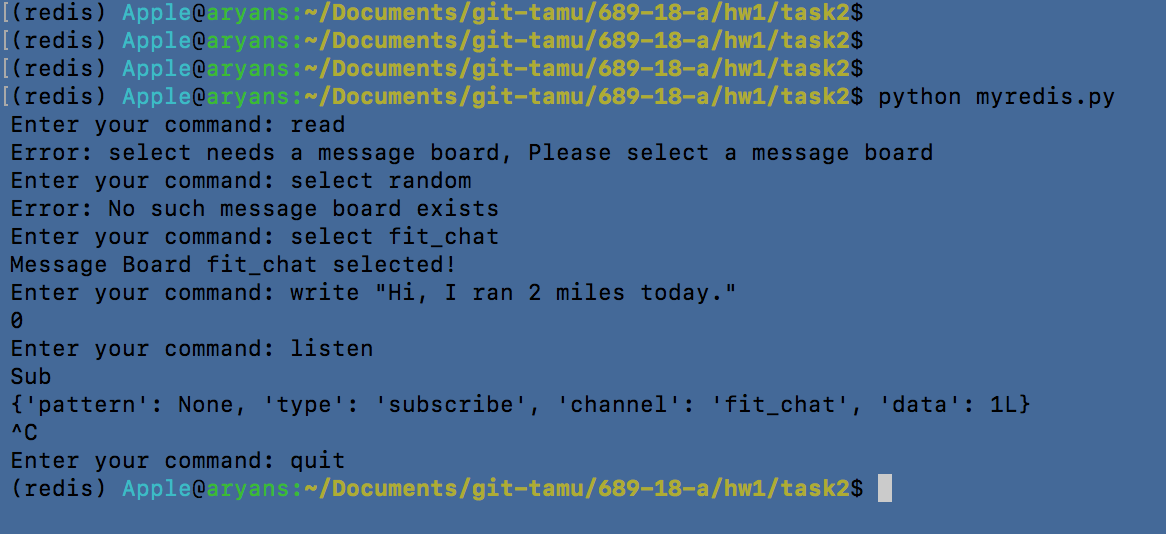
\includegraphics[width=1\textwidth]{2.png}
	\caption{\label{fig:data}Results for Task 2}
\end{figure}

\begin{figure}
	\centering
	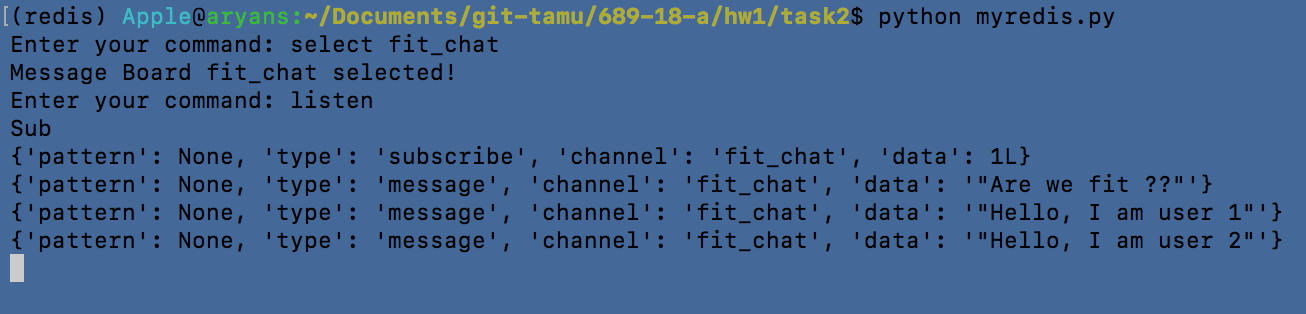
\includegraphics[width=1\textwidth]{3.png}
	\caption{\label{fig:data}Results for Task 2}
\end{figure}

\end{document}